\chapter{Introdução}
\label{chap:intro}

Segundo \citeonline{mamede2005}, as linhas de transmissão (LT) são elementos de um sistema elétrico que transportam a energia produzida pelas fontes de geração até as subestações abaixadoras instaladas próximas aos grandes centros de carga. Como as fontes de geração
de energia são construídas longes dos centros consumidores é preciso de linhas de transmissão de grandes extensões, o que as tornam susceptíveis às incidências de defeitos.

Um dos maiores problemas na distribuição de energia é o aquecimento anormal associado à alta resistência ou fluxo de corrente excessiva, onde alguns dos componentes afetados são o transformador trifásico, switches, conetores, fusíveis, cabos, etc \cite{canahuire}. Outro problema comum é a proximidade de objetos não desejados dos cabos de alta tensão, que podem acarretar em curtos no sistema elétrico de potência.

No Brasil, existe uma quantidade considerável de linhas de transmissão de alta tensão que já ultrapassaram a vida útil das quais foram destinadas. Com a degradação dos componentes nela instalados, vê-se a necessidade de manutenções preditivas a fim de verificar a integridade do sistema.

A técnica comumente utilizada para inspeção de linhas de transmissão é a termografia, capaz de identificar o aumento de temperatura nos cabos e equipamentos.  A inspeção por câmera térmica é de suma importância para a integridade dos equipamentos, já que por sua vez podem identificar possíveis problemas. Vale ressaltar que é necessário verificar as condições locais onde as torres estão instaladas, visto que construções e vegetação necessitam de uma distância mínima da mesma. 

Atualmente, a inspeção de linhas de transmissão é feita através de aeronaves tripuladas e uma equipe especializada. Essas inspeções são relativamente custosas e não possuem uma boa eficiência. Os helicópteros precisam sobrevoar próximos a LT para que um operado para realizar o procedimento, como pode ser vista na figura \ref{lineinspection}.

\pagebreak

\begin{figure}[!ht]
	\centering
	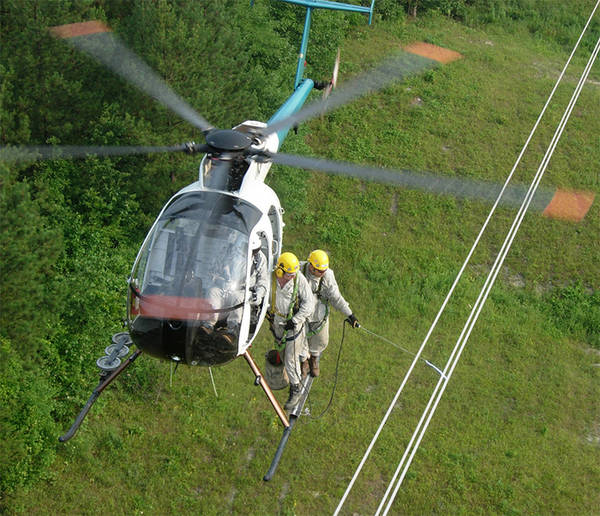
\includegraphics[width=10cm]{Figures/lineinpection.jpg}
	\caption{Inspeção de uma linha de transmissão} \label{lineinspection}
\end{figure}

Neste trabalho de conclusão de curso (TCC), seguindo a metodologia TheoPrax, é proposto o desenvolvimento da percepção de um robô móvel para inspeção de linhas de transmissão ELIR (Electrical Inspection Robot). O robô se irá se deslocar ao longo do cabo de alta tensão em busca de pontos quentes utilizando uma câmera térmica e verificando se há objetos próximos dos cabos com um sonar. Esses dados serão armazenados com a adição das coordenadas do robô fornecidas por um GPS e horário da detecção. O sistema irá conter outros sensores para compor toda a sua funcionalidade e serão abordados em mais detalhes nesse relatório.


%--------- NEW SECTION ----------------------
\section{Objetivos}
\label{sec:obj}

%Nesta se\c{c}\~ao os objetivos principal (tamb\'em
%pode-se se utilizar a palavra meta) da monografia de
%gradua\c{c}\~ao ou especializa\c{c}\~ao, disserta\c{c}\~ao de
%mestrado ou tese de doutorado s\~ao apresentados.

O objetivo deste trabalho é descrever os procedimentos realizados para construção do sistema de Percepção para um robô de inspeção de linhas de transmissão.  


\subsection{Objetivos Específicos}
\label{ssec:objesp}

%Nesta se\c{c}\~ao os objetivos espec\'ificos (tamb\'em
%pode-se se utilizar a palavra meta) da monografia de
%gradua\c{c}\~ao ou especializa\c{c}\~ao, disserta\c{c}\~ao %de
%mestrado ou tese de doutorado s\~ao apresentados.
\begin{itemize}
\item Realizar detecção de pontos quentes nas linhas de transmissão e em seus obstáculos;
\item Construir interface de comunicação com o usuário para apresentar as informações de segurança do robô, informação dos atuadores e todas as ocorrências da missão.
\end{itemize} 




%--------- NEW SECTION ----------------------
\section{Justificativa}
\label{sec:justi}

A garantia da disponibilidade de energia elétrica é um dos maiores problemas enfrentados pelas concessionárias de energia elétrica do país, pois além do custo elevado, a manutenção das linhas de transmissão é uma tarefa de alto risco para atividade humana. Atualmente, a inspeção é realizada a partir de aeronoves tripuladas ou com técnicos que apoiados a linha executam as tarefas com uma vestimenta especial com proteção para a indução.

A fim de reduzir o trabalho humano em atividades de risco muitos alternativas utilizando a robótica e o monitoramente térmico estão sendo utilizadas atualmente. O ELIR (Electrical Line Inspection Robot) foi idealizado para suprir a necessidade de segurança nas atividades de manutenção de linhas de alta tensão. Ele é um robô autônomo, que realiza o monitoramento de pontos quentes na linha a partir de imagem térmica, desta forma consiste em uma solução de manuntenção preditiva sem apresentar riscos a integridade física de funcionários.

O ELIR além de uma solução tecnológica é um trabalho acadêmico composto por estudantes de graduação, mestrado e doutorado da instituição. O desenvolvimento do protótipo para a instituição promove a atuação dos estudantes em robótica capacitando-os para a atuação na aŕea e cumprindo um dos principais objetivos da instituição que é o fomento a pesquisa e desenvolvimento. 

%--------- NEW SECTION ----------------------
\section{Requisitos do cliente}
\label{sec:reqc}
O desenvolvimento do sistema de percepção para o robô ELIR teve como fundamento os requisitos técnicos proposto pelo cliente do projeto. A descrição dos requisitos está mostrada abaixo:
    \subsection{Inspeção de Temperatura dos cabos, da estrutura e dos obstáculos} 
    Devem ser disponibilizadas as informações de medição de temperatura dos cabos, da estrutura da linha e de seus obstáculos. Esses dados devem ser obtidos através da câmera térmica para inspeção.    \subsection{Georreferenciamento dos eventos}
    Todos os eventos de detecção de pontos quentes, eventos de sobretemperatura e sobrecorrente devem ser sinalizados no arquivo de log informando a data, horário e localização através dos dados de latitude e longitude obtidos pelo GPS.
    \subsection{Disponibilizar vídeo dos eventos} 
    A inspeção realizada pela câmera térmica deve ser disponibilizada em tempo real na interface gráfica do robô.
    \subsection{Identificação de Posicionamento da garra no cabo} 
    A fim de garantir a confiabilidade da operação deve ser realizado um sensoriamento com o objetivo de verificar se as garras do robô estão devidamente amparadas no cabo da linha de alta tensão.
    \subsection{Inspeção de Linhas de Servidão}  
    Devem ser disponibilizadas informações de objetivos até 7m abaixo do robô
%--------- NEW SECTION ----------------------
\section{Organização do \thetypework}
\label{section:organizacao}

Este documento apresenta $x$ capítulos e está estruturado da seguinte forma:

\begin{itemize}

  \item \textbf{Capítulo \ref{chap:intro} - Introdução}: Contextualiza o âmbito, no qual a pesquisa proposta está inserida. Apresenta, portanto, a definição do problema, objetivos e justificativas da pesquisa e como este \thetypeworkthree está estruturado;

  \item \textbf{Capítulo \ref{chap:concep} - Conceito do Sistema}: Descreve como o sistema de Percepção é composto, apresenta a especificação técnica, a arquitetura geral do sistema, a arquitetura de software e os requisitos técnicos.;
  
  \item \textbf{Capítulo \ref{chap:mat} - Materiais e Métodos}: Apresenta os materiais utilizados no projeto, explica os suportes mecânicos criados, o diagrama elétrico e o desenho de placa desenvolvidos, apresenta as especificações de cada funcionalidade do sistema;
  
  \item \textbf{Capítulo \ref{chap:result} - Resultados}: Apresenta descrição dos testes unitários e integrados realizados;
 
  \item \textbf{Capítulo \ref{chap:conc} - Conclusão}: Apresenta as conclusóes, contribuições
  e algumas sugestões de atividades de pesquisa a serem desenvolvidas no futuro.

\end{itemize}
